% !TeX program = xelatex
\ifdefined\BookMaster\else
\documentclass[11pt,oneside]{article}
% !TeX program = xelatex
\usepackage[b5paper,left=22mm,right=22mm,top=20mm,bottom=22mm,footskip=11mm]{geometry}
\usepackage{fontspec}
\setmainfont{TeX Gyre Termes}
\setsansfont{TeX Gyre Heros}
\usepackage{amsmath,amssymb,mathtools,amsthm}
\renewcommand{\cdots}{\mathinner{\cdotp\cdotp\cdotp}}
\usepackage{graphicx,adjustbox,array,booktabs,longtable,multirow,enumitem,changepage,needspace}
\usepackage[table]{xcolor}
\usepackage{fancyhdr}
\raggedbottom
\interfootnotelinepenalty=10000
\newcommand{\BookFootnote}[2]{\begingroup\renewcommand{\thefootnote}{\fnsymbol{footnote}}\footnote[#1]{#2}\endgroup}
\newcommand{\BookFootnoteMark}[1]{\begingroup\renewcommand{\thefootnote}{\fnsymbol{footnote}}\footnotemark[#1]\endgroup}
\newcommand{\BookFootnoteText}[2]{\begingroup\renewcommand{\thefootnote}{\fnsymbol{footnote}}\footnotetext[#1]{#2}\endgroup}
\newenvironment{BookFloat}[1]{\par\addvspace{.6\baselineskip}\noindent\def\BookFloatID{#1}\begin{minipage}{\linewidth}\phantomsection\label{bookfloat:#1:start}}{\phantomsection\label{bookfloat:\BookFloatID:end}\end{minipage}\par\addvspace{.6\baselineskip}}

\usepackage[unicode,hidelinks]{hyperref}
\pagestyle{fancy}
\fancyhf{}
\newcommand{\BookFooter}{}
\fancyfoot[L]{\parbox[b]{\dimexpr\textwidth-15mm}{\footnotesize\BookFooter}}
\fancyfoot[R]{\footnotesize\thepage}
\renewcommand{\headrulewidth}{0pt}
\renewcommand{\footrulewidth}{0pt}
\setlength{\parindent}{0pt}
\setlength{\parskip}{0.2em}
\setlength{\emergencystretch}{3em}
\setlist{nosep,leftmargin=1.7em,labelsep=.65em}
\newif\ifBookNarrative
\BookNarrativetrue
\newenvironment{BookBody}{\setlength{\parindent}{0pt}}{}
\newcommand{\BookStatement}[1]{\par\addvspace{.6\baselineskip}\noindent #1\enspace\ignorespaces}
\newcommand{\BookLabel}[1]{\par\addvspace{.6\baselineskip}\needspace{3\baselineskip}\noindent\textbf{#1}\quad\ignorespaces}
\newcommand{\BookHeading}[1]{\par\addvspace{\baselineskip}\needspace{4\baselineskip}\noindent{\large\bfseries #1}\par\medskip}
\newcommand{\BookSubheading}[1]{\par\addvspace{.7\baselineskip}\needspace{3\baselineskip}\noindent{\bfseries #1}\par\smallskip}
\newcommand{\BookTextHeading}[1]{\par\addvspace{.7\baselineskip}\needspace{3\baselineskip}\noindent #1\par\smallskip}
\newcommand{\BookSectionTitle}[2]{\par\addvspace{1.2\baselineskip}\needspace{5\baselineskip}\noindent\colorbox{gray!25}{\sffamily\bfseries\small SECTION #1}\quad{\large\bfseries #2}\par\medskip}
\newcommand{\BookExerciseTitle}[1]{\par\addvspace{\baselineskip}\needspace{4\baselineskip}\noindent{\color{gray}\rule{1.5mm}{1.5mm}}\enspace{\large\bfseries Exercises #1}\par\medskip}
\newcommand{\BookBullet}[1]{\begin{list}{\textbullet}{\setlength{\leftmargin}{1.7em}\setlength{\labelwidth}{1em}\setlength{\labelsep}{.7em}\setlength{\topsep}{0pt}\setlength{\parsep}{0pt}\setlength{\itemsep}{0pt}}\item #1\end{list}}
\newcommand{\BookExercise}[2]{\begin{list}{\textbf{#1}}{\setlength{\leftmargin}{2.2em}\setlength{\labelwidth}{1.5em}\setlength{\labelsep}{.7em}\setlength{\topsep}{.15em}\setlength{\parsep}{0pt}\setlength{\itemsep}{0pt}}\item #2\end{list}}
\newcommand{\BookEnd}[1]{\unskip\nobreak\hfill\ensuremath{#1}}
\newcommand{\BookSource}[2]{\phantomsection\label{sourcepage:#1}} % Source-page anchors, retained through reflow.
\usepackage{multicol}
\usepackage{tikz}
\newcommand{\BookPartEntry}[2]{\par\noindent\makebox[17mm][l]{\bfseries Section #1}#2\par}
\newcommand{\BookPartTitle}[3]{\par\bigskip\noindent\begin{tikzpicture}\node[anchor=north west,inner sep=0pt,outer sep=0pt] (bookpart) at (0,0) {\begin{minipage}{\dimexpr\linewidth-.5pt}\hspace*{26mm}\begin{minipage}[t]{\dimexpr\linewidth-26mm}\begin{adjustbox}{max width=\linewidth}{\fontsize{20}{24}\selectfont\bfseries #2}\end{adjustbox}\par\vspace{6mm}\hrule\vspace{6mm}{\sffamily\footnotesize\setlength{\parskip}{.3em}#3}\vspace{3mm}\end{minipage}\end{minipage}};\path[shade,top color=gray!60,bottom color=white] (0,0) rectangle ([xshift=24mm]bookpart.south west);\node[anchor=north,font=\sffamily\bfseries\small] at (12mm,-2mm) {PART};\node[anchor=north,font=\sffamily\bfseries\Huge] at (12mm,-7mm) {#1};\end{tikzpicture}\par\bigskip}
\newsavebox{\BookMathBox}
\makeatletter
\newcommand{\BookInline}[1]{\leavevmode\hskip0pt\relax\begingroup\in@{\begin}{#1}\ifin@\sbox{\BookMathBox}{\(#1\)}\ifdim\wd\BookMathBox>\dimexpr\linewidth-1em\relax\resizebox{\dimexpr\linewidth-1em\relax}{!}{\usebox{\BookMathBox}}\else\(#1\)\fi\else\in@{\left}{#1}\ifin@\sbox{\BookMathBox}{\(#1\)}\ifdim\wd\BookMathBox>\dimexpr\linewidth-1em\relax\resizebox{\dimexpr\linewidth-1em\relax}{!}{\usebox{\BookMathBox}}\else\(#1\)\fi\else\(#1\)\fi\fi\endgroup\hskip0pt\relax}
\makeatother
\DeclareMathOperator{\Aut}{Aut}
\DeclareMathOperator{\End}{End}
\DeclareMathOperator{\Hom}{Hom}
\DeclareMathOperator{\GF}{GF}
\DeclareMathOperator{\irr}{irr}
\DeclareMathOperator{\lt}{lt}
\DeclareMathOperator{\lp}{lp}
\providecommand{\textcircled}[1]{\textnormal{(#1)}}

\begin{document}
\fi
\renewcommand{\BookFooter}{Section 3 Abelian Examples}
\pdfbookmark[0]{Section 3 Abelian Examples}{03_abelian_examples}
\ifdefined\BookMaster\else\setcounter{page}{32}\fi
% Source PDF page 49; original printed page 32
\BookSource{49}{32}
\BookNarrativetrue

\begin{BookBody}

\BookSectionTitle{3}{Abelian Examples}

\noindent In this section we introduce two families of abelian groups and one special abelian group. These groups will be very useful in our study of groups in that they provide examples we can use to help understand concepts and test conjectures. Furthermore, we will see that some of them arise frequently in the study of groups.

We start by defining the set \BookInline{\mathbb{Z}_{n}= \{0,\allowbreak 1,\allowbreak 2,\allowbreak 3,\allowbreak...,\allowbreak n- 1\},\allowbreak } the first \BookInline{n- 1} positive integers together with 0, which makes a total of \BookInline{n} elements. To define an operation \BookInline{+ _{n}} on \BookInline{\mathbb{Z}_{n},\allowbreak } we let \BookInline{a,\allowbreak b\in \mathbb{Z}_{n}.} Then

\begin{center}\begin{adjustbox}{max width=\linewidth}\BookInline{\displaystyle a + _ { n } b = \left\{ \begin{aligned} & a + b & \text { if } a + b < n \\ & a + b - n \text { if } a + b \geq n \end{aligned} \right. .}\end{adjustbox}\end{center}

Note that for any \BookInline{a,\allowbreak b\in \mathbb{Z}_{n},\allowbreak 0\leq a+ b\leq 2n- 2,\allowbreak } so \BookInline{0\leq a+ _{n}b\leq n- 1} is an operation which we call\textbf{ addition modulo} \BookInline{n.} Addition modulo \BookInline{n} is clearly commutative: \BookInline{a+ _{n}b= b+ _{n}a} for any \BookInline{a,\allowbreak b\in \mathbb{Z}_{n}.} The number 0 is an identity, the inverse of \BookInline{a\in \mathbb{Z}_{n}} is \BookInline{n- a} for \BookInline{a\neq 0,\allowbreak } and the inverse of 0 is 0. To show that \BookInline{\langle \mathbb{Z}_{n},\allowbreak + _{n}\rangle } is an abelian group, it only remains to show that \BookInline{+ _{n}} is associative. Although it is not difficult to show directly that \BookInline{+ _{n}} is associative, it is a little tedious, so we defer the proof until we develop the circle group and then use properties of that group to conclude that \BookInline{\langle \mathbb{Z}_{n},\allowbreak + _{n}\rangle } is an abelian group.

\BookLabel{3.1 Example} For \BookInline{n= 1,\allowbreak \mathbb{Z}_{1}= \{0\},\allowbreak } which is the trivial group with just one element. For \BookInline{n= 2,\allowbreak \mathbb{Z}_{2}= } \BookInline{\{0,\allowbreak 1\},\allowbreak } which as we saw in Section 2 is isomorphic with \BookInline{\{1,\allowbreak - 1\}} under multiplication. It is important to note that completely different operations on sets can still define isomorphic groups. We also saw in Section 2 that any group with exactly three elements is isomorphic with any other group with exactly three elements. Therefore \BookInline{\mathbb{Z}_{3}} under addition modulo 3 is isomorphic with the group consisting of the three matrices

\begin{center}\begin{adjustbox}{max width=\linewidth}\BookInline{\displaystyle \left\{ \left[ \begin{array} { l } 1 0 \\ 0 1 \end{array} \right] ,\allowbreak  \left[ \begin{array} { c } - \frac { 1 } { 2 } - \frac { \sqrt { 3 } } { 2 } \\ \frac { \sqrt { 3 } } { 2 } - \frac { 1 } { 2 } \end{array} \right] ,\allowbreak  \left[ \begin{array} { c } - \frac { 1 } { 2 } \frac { \sqrt { 3 } } { 2 } \\ - \frac { \sqrt { 3 } } { 2 } - \frac { 1 } { 2 } \end{array} \right] \right\}}\end{adjustbox}\end{center}

\noindent under matrix multiplication. Again we see that two groups can be isomorphic, but have completely different sets and operations\BookInline{.}\BookEnd{\blacktriangle}

\BookLabel{3.2 Example} 

Let us look more closely at the group table for \BookInline{\mathbb{Z}_{4},\allowbreak } Table 3.3. We see that the inverse for 0 is 0, the inverse for 1 is \BookInline{4- 1= 3,\allowbreak } and the inverse for 2 is \BookInline{4- 2= 2.} In Exercise 20 in Section 2, you were asked to show that there are two groups with exactly four elements. The other group is the\textbf{ Klein 4-group} denoted \BookInline{V,\allowbreak } which stands for Vier, German for “four.” The group table for \BookInline{V} is displayed as Table 3.4. How can we tell that the two groups \BookInline{\mathbb{Z}_{4}} and \BookInline{V} are not isomorphic? We could try all possible one-to-one functions from \BookInline{\mathbb{Z}_{4}} onto \BookInline{K_{4}} to see if any of them make the table for \BookInline{\mathbb{Z}_{4}} look like the table for \BookInline{K_{4}.} This is tedious, so instead we look for a sneaky method. Notice that the diagonal entries of the table for \BookInline{K_{4}} are all the identity. No matter how we relabel

\begin{BookFloat}{03_abelian_examples-p49-11}
\begin{center}
\begin{minipage}[t]{0.4920\linewidth}\vspace{0pt}\begin{center}\small\textbf{3.3 Table}\end{center}
\begin{center}\begin{adjustbox}{max width=\linewidth}
\renewcommand{\arraystretch}{1.2}\setlength{\tabcolsep}{5pt}
\begin{tabular}{cc|cccc}
\BookInline{\mathbb{Z}_{4}:} & \BookInline{+ _{4}} & 0 & 1 & 2 & 3\\\hline
 & 0 & 0 & 1 & 2 & 3\\
 & 1 & 1 & 2 & 3 & 0\\
 & 2 & 2 & 3 & 0 & 1\\
 & 3 & 3 & 0 & 1 & 2\\
\end{tabular}
\end{adjustbox}\end{center}\end{minipage}\hfill\begin{minipage}[t]{0.4255\linewidth}\vspace{0pt}\begin{center}\small\textbf{3.4 Table}\end{center}
\begin{center}\begin{adjustbox}{max width=\linewidth}
\renewcommand{\arraystretch}{1.2}\setlength{\tabcolsep}{5pt}
\begin{tabular}{cc|cccc}
\BookInline{V:} & \BookInline{\ast } & \BookInline{e} & \BookInline{a} & \BookInline{b} & \BookInline{c}\\\hline
 & \BookInline{e} & \BookInline{e} & \BookInline{a} & \BookInline{b} & \BookInline{c}\\
 & \BookInline{a} & \BookInline{a} & \BookInline{e} & \BookInline{c} & \BookInline{b}\\
 & \BookInline{b} & \BookInline{b} & \BookInline{c} & \BookInline{e} & \BookInline{a}\\
 & \BookInline{c} & \BookInline{c} & \BookInline{b} & \BookInline{a} & \BookInline{e}\\
\end{tabular}
\end{adjustbox}\end{center}\end{minipage}
\end{center}
\end{BookFloat}

\end{BookBody}

% Source PDF page 50; original printed page 33
\BookSource{50}{33}
\BookNarrativetrue

\begin{BookBody}

\noindent the entries in the table for \BookInline{\mathbb{Z}_{4},\allowbreak } only two entries along the diagonal will be the same. Therefore \BookInline{\mathbb{Z}_{4}} and \BookInline{K_{4}} are not isomorphic\BookInline{.}\BookEnd{\blacktriangle}

Looking back at the definition of \BookInline{+ _{n}} there is no reason we had to restrict our set to integers \BookInline{a} with \BookInline{0\leq a<n.} In fact, the same formula defines an operation on all real numbers \BookInline{a} with \BookInline{0\leq a<n.} In general, let \BookInline{c} be any positive real number and \BookInline{a,\allowbreak b\in [0,\allowbreak c).} We define \BookInline{+ _{c}} by

\begin{center}\begin{adjustbox}{max width=\linewidth}\BookInline{\displaystyle a + _ { c } b = \left\{ \begin{aligned} & a + b & \text { if } a + b < c \\ & a + b - c \text { if } a + b \geq c \end{aligned} \right. .}\end{adjustbox}\end{center}

\noindent This operation is called\textbf{ addition modulo} \BookInline{c.} It is easy to see that addition modulo \BookInline{c} is an operation on \BookInline{[0,\allowbreak c),\allowbreak } it is commutative, 0 is an identity, the inverse of 0 is 0, and the inverse of any \BookInline{a\in (0,\allowbreak c)} is \BookInline{c- a.} Instead of writing \BookInline{[0,\allowbreak c)} we will denote this set as \BookInline{\mathbb{R}_{c}.} In order to show that \BookInline{\langle \mathbb{R}_{c},\allowbreak + _{c}\rangle } is an abelian group, it remains to show that \BookInline{+ _{c}} is associative. Again, we defer the proof until after we develop the circle group.

\BookLabel{3.5 Example} Let \BookInline{c= 2\pi.} Then \BookInline{\frac { 2 } { 5 } \pi + _ { 2 \pi } \frac { 6 } { 5 } \pi = \frac { 8 } { 5 } \pi} and \BookInline{\frac { 7 } { 5 } \pi + _ { 2 \pi } \frac { 6 } { 5 } \pi = \frac { 3 } { 5 } \pi}. The inverse of \BookInline{\frac{\pi }{2}} is \BookInline{2\pi - } \BookInline{\textstyle { \frac { \pi } { 2 } } = { \frac { 3 } { 2 } } \pi} \BookInline{.}\BookEnd{\blacktriangle}

In the group \BookInline{\langle \mathbb{R}_{2\pi },\allowbreak + _{2\pi }\rangle,\allowbreak } we are essentially equating 0 with \BookInline{2\pi } in the sense that if \BookInline{a} and \BookInline{b} add to give \BookInline{2\pi,\allowbreak } we know that \BookInline{a+ _{2\pi }b= 0.} Intuitively, we can think of this geometrically as taking a string of length \BookInline{2\pi } and attaching the ends together to form a circle of radius 1. Our next goal is to make this idea more precise by defining a group on the unit circle in the plane and showing that this group is isomorphic with \BookInline{\mathbb{R}_{2\pi }.} To do this, we first review some facts about complex numbers.

\begin{BookFloat}{03_abelian_examples-p50-6}
\begin{center}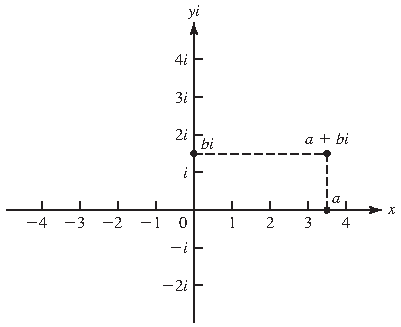
\includegraphics[width=0.550\linewidth,height=.8\textheight,keepaspectratio]{assets/p050_07.pdf}\end{center}
\begin{center}\small\textbf{3.6 Figure}\end{center}
\end{BookFloat}

\BookTextHeading{\textbf{Complex Numbers}  }

\noindent A real number can be visualized geometrically as a point on a line that we often regard as an \BookInline{x-}axis. A complex number can be regarded as a point in the Euclidean plane, as shown in Fig. 3.6. Note that we label the vertical axis as the \BookInline{yi-}axis rather than just the \BookInline{y-}axis, and label the point one unit above the origin with \BookInline{i} rather than 1. The point with Cartesian coordinates \BookInline{(a,\allowbreak b)} is labeled \BookInline{a+ } \textit{bi} in Fig. 3.6. The set \BookInline{\mathbb{C}} of\textbf{ complex numbers} is defined by

\begin{center}\begin{adjustbox}{max width=\linewidth}\BookInline{\displaystyle \mathbb{C}= \{a+ bi\mid a,\allowbreak b\in \mathbb{R}\}.}\end{adjustbox}\end{center}

\noindent We consider \BookInline{\mathbb{R}} to be a subset of the complex numbers by identifying a real number \BookInline{r} with the complex number \BookInline{r+ 0i.} For example, we write \BookInline{3+ 0i} as 3 and \BookInline{- \pi + 0i} as \BookInline{- \pi } and \BookInline{0+ 0i} as 0. Similarly, we write \BookInline{0+ 1i} as \BookInline{i} and \BookInline{0+ si} as \BookInline{si.}

\end{BookBody}

% Source PDF page 51; original printed page 34
\BookSource{51}{34}
\BookNarrativetrue

\begin{BookBody}

Complex numbers were developed after the development of real numbers. The complex number \BookInline{i} was\textit{ invented} to provide a solution to the quadratic equation \BookInline{x^{2}= - 1,\allowbreak } so we require that

\begin{center}\begin{adjustbox}{max width=\linewidth}\BookInline{\displaystyle i^{2}= - 1.(1)}\end{adjustbox}\end{center}

\noindent Unfortunately\BookInline{,\allowbreak i} has been called an\textbf{ imaginary number,} and this terminology has led generations of students to view the complex numbers with more skepticism than the real numbers. Actually,\textit{ all} numbers, such as \BookInline{1,\allowbreak 3,\allowbreak \pi,\allowbreak - \sqrt{3},\allowbreak } and \BookInline{i} are inventions of our minds. There is no physical entity that\textit{ is} the number 1. If there were, it would surely be in a place of honor in some great scientific museum, and past it would file a steady stream of mathematicians, gazing at 1 in wonder and awe. A basic goal of this text is to show how we can invent solutions of polynomial equations when the coefficients of the polynomial may not even be real numbers!

\BookTextHeading{\textbf{Multiplication of Complex Numbers}  }

\noindent The product \BookInline{(a+ } \textit{bi}\BookInline{)(c+ } \textit{di}) is defined in the way it must be if we are to enjoy the familiar properties of real arithmetic and require that \BookInline{i^{2}= - 1,\allowbreak } in accord with Eq. (1). Namely, we see that we want to have

\begin{center}\begin{adjustbox}{max width=\linewidth}\BookInline{\displaystyle \begin{aligned}(a+ bi)(c+ di)&= ac+ adi+ bci+ bdi^{2} \\ &= ac+ adi+ bci+ bd(- 1) \\ &= (ac- bd)+ (ad+ bc)i.\end{aligned}}\end{adjustbox}\end{center}

\noindent Consequently, we define multiplication of \BookInline{z_{1}= a+ } \textit{bi} and \BookInline{z_{2}= c+ } \textit{di} as

\begin{center}\begin{adjustbox}{max width=\linewidth}\BookInline{\displaystyle z_{1}z_{2}= (a+ bi)(c+ di)= (ac- bd)+ (ad+ bc)i,\allowbreak (2)}\end{adjustbox}\end{center}

\noindent which is of the form \BookInline{r+ si} with \BookInline{r= } \textit{ac} \BookInline{- bd} and \BookInline{s= ad+ bc.} It is routine to check that the usual properties \BookInline{z_{1}z_{2}= z_{2}z_{1}(}commutative\BookInline{),\allowbreak z_{1}(z_{2}z_{3})= (z_{1}z_{2})z_{3}(}associative), and \BookInline{z_{1}(z_{2}+ z_{3})= z_{1}z_{2}+ z_{1}z_{3}(}distributive) all hold for all \BookInline{z_{1},\allowbreak z_{2},\allowbreak z_{3}\in \mathbb{C}.}

\BookLabel{3.7 Example} 

\BookTextHeading{Compute (2 \ensuremath{-} 5\textit{i})(8 + 3\textit{i}).  }

\BookLabel{\textit{Solution}} We don’t memorize Eq. (2), but rather we compute the product as we did to motivate that equation. We have

\begin{center}\begin{adjustbox}{max width=\linewidth}\BookInline{\displaystyle (2- 5i)(8+ 3i)= 16+ 6i- 40i+ 15= 31- 34i.\blacktriangle}\end{adjustbox}\end{center}

\noindent To establish the geometric meaning of complex multiplication, we first define the\textbf{ abso}\textbf{lute value} \BookInline{|a+ } \textit{bi}\BookInline{|} of \BookInline{a+ } \textit{bi} by

\begin{center}\begin{adjustbox}{max width=\linewidth}\BookInline{\displaystyle |a+ bi|= \sqrt{a^{2}}+ b^{2}.}\end{adjustbox}\end{center}

\noindent This absolute value is a nonnegative real number and is the distance from \BookInline{a+ } \textit{bi} to the origin in Fig. 3.6. We can now describe a complex number \BookInline{z} in the polar-coordinate form

\begin{center}\begin{adjustbox}{max width=\linewidth}\BookInline{\displaystyle z= |z|(\;\text{cos}\;\theta + i\;\text{sin}\;\theta ),\allowbreak (4)}\end{adjustbox}\end{center}

\noindent where \BookInline{\theta } is the angle measured counterclockwise from the positive \BookInline{x-}axis to the vector from 0 to \BookInline{z,\allowbreak } as shown in Fig. 3.8. A famous formula due to Leonard Euler states that

\begin{center}\begin{adjustbox}{max width=\linewidth}\BookInline{\displaystyle e^{i\theta }= \;\text{cos}\;\theta + i\;\text{sin}\;\theta .}\end{adjustbox}\end{center}

\begin{center}\begin{adjustbox}{max width=\linewidth}\BookInline{\displaystyle \;\text{Euler}\;\text{’}\;\text{s Formula}\;}\end{adjustbox}\end{center}

\end{BookBody}

% Source PDF page 52; original printed page 35
\BookSource{52}{35}
\BookNarrativetrue

\begin{BookBody}

\begin{BookFloat}{03_abelian_examples-p52-0}
\begin{center}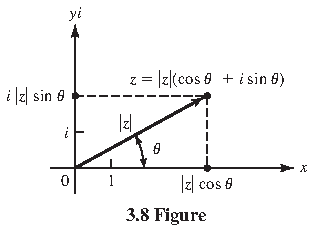
\includegraphics[width=0.427\linewidth,height=.8\textheight,keepaspectratio]{assets/p052_01.pdf}\end{center}
\end{BookFloat}

\noindent We ask you to derive Euler’s formula formally from the power series expansions for \BookInline{e^{\theta },\allowbreak } cos \BookInline{\theta,\allowbreak } and sin \BookInline{\theta } in Exercise 43. Using this formula, we can express \BookInline{z} in Eq. (4) as \BookInline{z= |z|e^{i\theta }.} Let us set

\begin{center}\begin{adjustbox}{max width=\linewidth}\BookInline{\displaystyle z_{1}= |z_{1}|e^{i\theta _{1}}\;\text{and}\;z_{2}= |z_{2}|e^{i\theta _{2}}}\end{adjustbox}\end{center}

\noindent and compute their product in this form, assuming that the usual laws of exponentiation hold with complex number exponents. We obtain

\begin{center}\begin{adjustbox}{max width=\linewidth}\BookInline{\displaystyle \begin{aligned}z_{1}z_{2}&= |z_{1}|e^{i\theta _{1}}|z_{2}|e^{i\theta _{2}}= |z_{1}||z_{2}|e^{i(\theta _{1}+ \theta _{2})} \\ &= |z_{1}||z_{2}|[\;\text{cos}\;(\theta _{1}+ \theta _{2})+ i\;\text{sin}\;(\theta _{1}+ \theta _{2})].(5)\end{aligned}}\end{adjustbox}\end{center}

\noindent Note that Eq. 5 concludes in the polar form of Eq. 4 where \BookInline{|z_{1}z_{2}|= |z_{1}||z_{2}|} and the polar angle \BookInline{\theta } for \BookInline{z_{1}z_{2}} is the sum \BookInline{\theta = \theta _{1}+ \theta _{2}.} Thus, geometrically, we multiply complex numbers by multiplying their absolute values and adding their polar angles, as shown in Fig. 3.9. Exercise 41 indicates how this can be derived via trigonometric identities without recourse to Euler’s formula and assumptions about complex exponentiation.

\begin{BookFloat}{03_abelian_examples-p52-6}
\begin{center}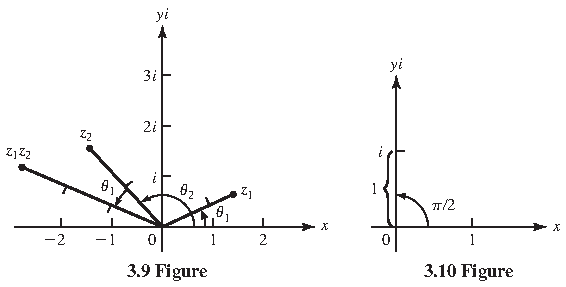
\includegraphics[width=0.777\linewidth,height=.8\textheight,keepaspectratio]{assets/p052_00.pdf}\end{center}
\end{BookFloat}

Note that \BookInline{i} has polar angle \BookInline{\pi /2} and absolute value 1, as shown in Fig. 3.10. Thus \BookInline{i^{2}} has polar angle \BookInline{2(\pi /2)= \pi } and \BookInline{|1\cdot 1|= 1,\allowbreak } so that \BookInline{i^{2}= - 1.}

\BookLabel{3.11 Example} Find all solutions in \BookInline{\mathbb{C}} of the equation \BookInline{z^{2}= i.}

\BookLabel{\textit{Solution}} Writing the equation \BookInline{z^{2}= i} in polar form and using Eq. (5), we obtain

\begin{center}\begin{adjustbox}{max width=\linewidth}\BookInline{\displaystyle |z|^{2}(\;\text{cos}\;2\theta + i\;\text{sin}\;2\theta )= 1(0+ i).}\end{adjustbox}\end{center}

\noindent Thus \BookInline{|z|^{2}= 1,\allowbreak } so \BookInline{|z|= 1.} The angle \BookInline{\theta } for \BookInline{z} must satisfy cos \BookInline{2\theta = 0} and sin \BookInline{2\theta = 1.} Consequently\BookInline{,\allowbreak 2\theta = (\pi /2)+ n(2\pi ),\allowbreak } so \BookInline{\theta = (\pi /4)+ n\pi } for an integer \BookInline{n.} The values of

\end{BookBody}

% Source PDF page 53; original printed page 36
\BookSource{53}{36}
\BookNarrativetrue

\begin{BookBody}

\noindent \BookInline{n} yielding values \BookInline{\theta } where \BookInline{0\leq \theta <2\pi } are 0 and 1, yielding \BookInline{\theta = \pi /4} or \BookInline{\theta = 5\pi /4.} Our solutions are

\begin{center}\begin{adjustbox}{max width=\linewidth}\BookInline{\displaystyle z _ { 1 } = 1 \Bigg ( \cos \frac { \pi } { 4 } + i \sin \frac { \pi } { 4 } \Bigg ) \qquad \mathrm { a n d } \qquad z _ { 2 } = 1 \Bigg ( \cos \frac { 5 \pi } { 4 } + i \sin \frac { 5 \pi } { 4 } \Bigg )}\end{adjustbox}\end{center}

\noindent or

\begin{center}\begin{adjustbox}{max width=\linewidth}\BookInline{\displaystyle z _ { 1 } = \frac { 1 } { \sqrt { 2 } } ( 1 + i ) \qquad \mathrm { a n d } \qquad z _ { 2 } = \frac { - 1 } { \sqrt { 2 } } ( 1 + i ) .}\end{adjustbox}\end{center} \BookEnd{\blacktriangle}

\BookLabel{3.12 Example} Find all solutions of \BookInline{z^{4}= - 16.}

\BookLabel{\textit{Solution}} As in Example 3.11 we write the equation in polar form, obtaining

\begin{center}\begin{adjustbox}{max width=\linewidth}\BookInline{\displaystyle |z|^{4}(\;\text{cos}\;4\theta + i\;\text{sin}\;4\theta )= 16(- 1+ 0i).}\end{adjustbox}\end{center}

\noindent Consequently\BookInline{,\allowbreak |z|^{4}= 16,\allowbreak } so \BookInline{|z|= 2} while cos \BookInline{4\theta = - 1} and sin \BookInline{4\theta = 0.} We find that \BookInline{4\theta = \pi + n(2\pi ),\allowbreak } so \BookInline{\theta = (\pi /4)+ n(\pi /2)} for integers \BookInline{n.} The different values of \BookInline{\theta } obtained where \BookInline{0\leq \theta <2\pi } are \BookInline{\pi /4,\allowbreak 3\pi /4,\allowbreak 5\pi /4,\allowbreak } and \BookInline{7\pi /4.} Thus one solution of \BookInline{z^{4}= - 16} is

\begin{center}\begin{adjustbox}{max width=\linewidth}\BookInline{\displaystyle 2\bigg(\cos\frac{\pi}{4}+i\sin\frac{\pi}{4}\bigg)=2\bigg(\frac{1}{\sqrt{2}}+\frac{1}{\sqrt{2}}i\bigg)=\sqrt{2}(1+i).}\end{adjustbox}\end{center}

\noindent In a similar way, we find three more solutions,

\begin{center}\begin{adjustbox}{max width=\linewidth}\BookInline{\displaystyle \sqrt{2}(- 1+ i),\allowbreak \sqrt{2}(- 1- i),\allowbreak \;\text{and}\;\sqrt{2}(1- i).}\end{adjustbox}\end{center} \BookEnd{\blacktriangle}

The last two examples illustrate that we can find solutions of an equation \BookInline{z^{n}= } \BookInline{a+ } \textit{bi} by writing the equation in polar form. There will always be \BookInline{n} solutions, provided that \BookInline{a+ } \textit{bi}\BookInline{\neq 0.} Exercises 16 through 21 ask you to solve equations of this type.

We will not use addition or division of complex numbers, but we probably should mention that addition is given by

\begin{center}\begin{adjustbox}{max width=\linewidth}\BookInline{\displaystyle (a+ bi)+ (c+ di)= (a+ c)+ (b+ d)i.(6)}\end{adjustbox}\end{center}

\noindent and division of \BookInline{a+ } \textit{bi} by nonzero \BookInline{c+ } \textit{di} can be performed using only division of real numbers as follows:

\begin{center}\begin{adjustbox}{max width=\linewidth}\BookInline{\displaystyle \begin{aligned}\frac{a + bi}{c + di} &= \frac{a + bi}{c + di} \cdot \frac{c - di}{c - di} = \frac{(ac + bd) + (bc - ad)i}{c^2 + d^2} \\&= \frac{ac + bd}{c^2 + d^2} + \frac{bc - ad}{c^2 + d^2}i.\end{aligned}}\end{adjustbox}\end{center}

\begin{BookFloat}{03_abelian_examples-p53-18}
\begin{center}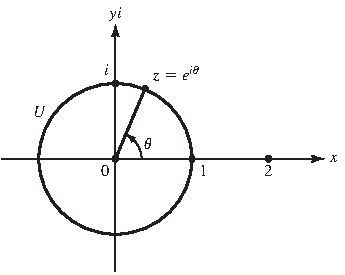
\includegraphics[width=0.473\linewidth,height=.8\textheight,keepaspectratio]{assets/p053_19.pdf}\end{center}
\begin{center}\small\textbf{3.13 Figure}\end{center}
\end{BookFloat}

\end{BookBody}

% Source PDF page 54; original printed page 37
\BookSource{54}{37}
\BookNarrativetrue

\begin{BookBody}

\BookTextHeading{\textbf{Algebra on the Unit Circle}  }

\noindent Let \BookInline{U= \{z\in \mathbb{C}\mid |z|= 1\},\allowbreak } so that \BookInline{U} is the circle in the Euclidean plane with center at the origin and radius 1, as shown in Fig. 3.13.

\BookLabel{3.14 Theorem} \BookInline{\langle U,\allowbreak \cdot \rangle } is an abelian group.

\BookLabel{\textit{Proof}} We first check that \BookInline{U} is closed under multiplication. Let \BookInline{z_{1},\allowbreak z_{2}\in U.} Then \BookInline{|z_{1}|= |z_{2}|= 1,\allowbreak } which implies that \BookInline{|z_{1}z_{1}|= 1,\allowbreak } showing \BookInline{z_{1}z_{2}\in U.}

Since multiplication of complex numbers is associative and commutative in general, multiplication in \BookInline{U} is also associative and commutative, which verifies \BookInline{\mathcal{G}_{1}} and the condition for abelian.

The number \BookInline{1\in U} is the identity, verifying condition \BookInline{\mathcal{G}_{2}.}

For each \BookInline{a+ } \textit{bi} \BookInline{\in U,\allowbreak }

\begin{center}\begin{adjustbox}{max width=\linewidth}\BookInline{\displaystyle (a+ bi)(a- bi)= a^{2}- (bi)^{2}= a^{2}+ b^{2}= |a+ bi|^{2}= 1.}\end{adjustbox}\end{center}

\noindent So the inverse of \BookInline{a+ } \textit{bi} is \BookInline{a- } \textit{bi}, which verifies condition \BookInline{\mathcal{G}_{3}.} Thus \BookInline{U} is an abelian group under multiplication\BookInline{.}\BookEnd{\blacklozenge}

Figure 3.13 gives us a way of relabeling points in \BookInline{U} as points in \BookInline{\mathbb{R}_{2\pi }.} We simply relabel \BookInline{z} as \BookInline{\theta } where \BookInline{0\leq \theta <2\pi.} Let \BookInline{f:U\to \mathbb{R}_{2\pi }} be given by \BookInline{f(z)= \theta } according to this relabeling. Then for \BookInline{z_{1},\allowbreak z_{2}\in U,\allowbreak f(z_{1}z_{2})= f(z_{1})+ _{2\pi }f(z_{2})} since multiplying in \BookInline{U} simply adds the corresponding angles:

\begin{center}\begin{adjustbox}{max width=\linewidth}\BookInline{\displaystyle \;\text{if}\;z_{1}\leftrightarrow \theta _{1}\;\text{and}\;z_{2}\leftrightarrow \theta _{2},\allowbreak \;\text{then}\;z_{1}\cdot z_{2}\leftrightarrow (\theta _{1}+ _{2\pi }\theta _{2}).(8)}\end{adjustbox}\end{center}

\noindent Recall that all that remains to show that \BookInline{\mathbb{R}_{2\pi }} is a group is to show that \BookInline{+ _{2\pi }} is associative. Since the operations of multiplication in \BookInline{U} and addition modulo \BookInline{2\pi } in \BookInline{\mathbb{R}_{2\pi }} are the same using the above relabeling and multiplication in \BookInline{U} is associative, addition modulo \BookInline{2\pi } is also associative. This completes the proof that \BookInline{\langle \mathbb{R}_{2\pi },\allowbreak + _{2\pi }\rangle } is a group. Furthermore, the relabeling (8) shows that the two groups \BookInline{\langle U,\allowbreak \cdot \rangle } and \BookInline{\langle \mathbb{R}_{2\pi },\allowbreak + _{2\pi }\rangle } are isomorphic. In Exercise 45, you will be asked to prove that for any \BookInline{b>0} and \BookInline{c>0,\allowbreak \langle \mathbb{R}_{b},\allowbreak + _{b}\rangle } is an abelian group and \BookInline{\langle \mathbb{R}_{b},\allowbreak + _{b}\rangle \simeq \langle \mathbb{R}_{c},\allowbreak + _{c}\rangle.} Since \BookInline{\langle \mathbb{R}_{2\pi },\allowbreak + _{2\pi }\rangle } is isomorphic with \BookInline{\langle U,\allowbreak \cdot \rangle,\allowbreak } for every \BookInline{c>0,\allowbreak \langle \mathbb{R}_{c},\allowbreak + _{c}\rangle } is also isomorphic with \BookInline{\langle U,\allowbreak \cdot \rangle,\allowbreak } meaning they have the same algebraic properties.

\BookLabel{3.15 Example} The equation \BookInline{z\cdot z\cdot z\cdot z= 1} in \BookInline{U} has exactly four solutions, namely\BookInline{,\allowbreak 1,\allowbreak i,\allowbreak - 1,\allowbreak } and \BookInline{- i.} Now \BookInline{1\in U} and \BookInline{0\in \mathbb{R}_{2\pi }} correspond, and the equation \BookInline{x+ _{2\pi }x+ _{2\pi }x+ _{2\pi }x= 0} in \BookInline{\mathbb{R}_{2\pi }} has exactly four solutions, namely\BookInline{,\allowbreak 0,\allowbreak \pi /2,\allowbreak \pi,\allowbreak } and \BookInline{3\pi /2,\allowbreak } which, of course, correspond to \BookInline{1,\allowbreak i,\allowbreak - 1,\allowbreak } and \BookInline{- i,\allowbreak } respectively\BookInline{.}\BookEnd{\blacktriangle}

\BookTextHeading{\textbf{Roots of Unity}  }

\noindent The elements of the set \BookInline{U_{n}= \{z\in \mathbb{C}\mid z^{n}= 1\}} are called the \BookInline{n}th\textbf{ roots of unity}. In Exercise 46 you are asked to prove that \BookInline{U_{n}} is a group under multiplication. Using the techniques from Examples 3.11 and 3.12, we see that the elements of this set are the numbers \BookInline{2\pi 2\pi }

\begin{center}\begin{adjustbox}{max width=\linewidth}\BookInline{\displaystyle e ^ { \left( m { \frac { 2 \pi } { n } } \right) i } = \cos \left( m { \frac { 2 \pi } { n } } \right) + i \sin \left( m { \frac { 2 \pi } { n } } \right) \quad { \mathrm { f o r } } \; m = 0 ,\allowbreak  1 ,\allowbreak  2 ,\allowbreak  \ldots ,\allowbreak  n - 1 .}\end{adjustbox}\end{center}

\noindent They all have absolute value 1, so \BookInline{U_{n}\subset U.} If we let \BookInline{\zeta = } cos \BookInline{2n\pi + i} sin \BookInline{2n\pi,\allowbreak } then these \BookInline{n}th roots of unity can be written as

\begin{center}\begin{adjustbox}{max width=\linewidth}\BookInline{\displaystyle 1= \zeta ^{0},\allowbreak \zeta ^{1},\allowbreak \zeta ^{2},\allowbreak \zeta ^{3},\allowbreak \cdots ,\allowbreak \zeta ^{n- 1}.(9)}\end{adjustbox}\end{center}

\noindent Because \BookInline{\zeta ^{n}= 1,\allowbreak } these \BookInline{n} powers of \BookInline{\zeta } are closed under multiplication. For example, with \BookInline{n= 10,\allowbreak } we have 6 8 14 10 4 4 4 \BookInline{\zeta \zeta = \zeta = \zeta \zeta = 1\cdot \zeta = \zeta.}

\end{BookBody}

% Source PDF page 55; original printed page 38
\BookSource{55}{38}
\BookNarrativetrue

\begin{BookBody}

\noindent Thus we see that we can compute \BookInline{\zeta ^{i}\zeta ^{j}} by computing \BookInline{i+ _{n}j,\allowbreak } viewing \BookInline{i} and \BookInline{j} as elements of \BookInline{\mathbb{Z}_{n}.}

By relabeling an element \BookInline{\zeta ^{m}\in U_{n}} to \BookInline{m\in \mathbb{Z}_{n}} we can see that addition modulo \BookInline{n} in \BookInline{\mathbb{Z}_{n}} is also associative, which completes the proof that \BookInline{\langle \mathbb{Z}_{n},\allowbreak + _{n}\rangle } is an abelian group.

\BookLabel{3.16 Example} We solve the equation \BookInline{x+ _{8}x+ _{8}x= 1} in \BookInline{\mathbb{Z}_{8}} using trial and error. We note that neither 0, 1, nor 2 is a solution simply by substitution. However, substituting \BookInline{x= 3} gives \BookInline{3+ _{8}3+ _{8}3= 6+ _{8}3= 1,\allowbreak } which shows \BookInline{x= 3} is a solution. We can also check by substituting that neither 4, 5, 6, nor 7 are solutions. So the only solution is \BookInline{x= 3.} Because \BookInline{\mathbb{Z}_{8}} is isomorphic with \BookInline{U_{8}} by the correspondence \BookInline{k\in \mathbb{Z}_{8}} corresponds with \BookInline{\zeta ^{k},\allowbreak } the corresponding equation in \BookInline{U_{8}} is \BookInline{z \cdot z \cdot z = \zeta = e ^ { \frac { 2 \pi } { 8 } i }}. Without further calculations we know that there is only one solution to \BookInline{z\cdot z\cdot z= \zeta } in \BookInline{U_{8}} and that solution is \BookInline{z = \zeta^{3} = e^{3\frac{2\pi}{8}i} = \cos(6\pi/8) + i\sin(6\pi/8) = -\frac{\sqrt{2}}{2} + \frac{\sqrt{2}}{2}i} since this is the corresponding solution in \BookInline{\mathbb{Z}_{8}.}

There are three solutions to \BookInline{z^{3}= \zeta } in \BookInline{U.} We leave it to the reader to find the solutions and check that only one of them\BookInline{,\allowbreak \zeta ^{3},\allowbreak } is in \BookInline{U_{8}.}\BookEnd{\blacktriangle}

\noindent We summarize the results of this section.

\BookExercise{1.}{For any \BookInline{n\in \mathbb{Z}^{+ },\allowbreak \mathbb{Z}_{n}} is an abelian group under addition modulo \BookInline{n.}}

\BookExercise{2.}{For any \BookInline{n\in \mathbb{Z}^{+ },\allowbreak \mathbb{Z}_{n}} is isomorphic with \BookInline{U_{n},\allowbreak } an abelian group under complex number multiplication.}

\BookExercise{3.}{For any \BookInline{c>0,\allowbreak R_{c}} under addition modulo \BookInline{c} is a group.}

\BookExercise{4.}{\BookInline{U} under multiplication is a group.}

\BookExercise{5.}{For any \BookInline{c\in \mathbb{R}^{+ },\allowbreak \mathbb{R}_{c}} under addition modulo \BookInline{c} is isomorphic with \BookInline{U} under multiplication.}

\end{BookBody}

\BookNarrativefalse

\begin{BookBody}

\BookExerciseTitle{3} \BookEnd{\blacksquare}

\noindent In Exercises 1 through 9 compute the given arithmetic expression and give the answer in the form \BookInline{a+ } \textit{bi} for \BookInline{a,\allowbreak b\in \mathbb{R}.}

\BookExercise{1.}{\BookInline{i^{3}}}

\BookExercise{2.}{\BookInline{i^{4}}}

\BookExercise{3.}{26 \BookInline{i}}

\BookExercise{4.}{\BookInline{(- i)^{39}}}

\BookExercise{5.}{\BookInline{(3- 2i)(6+ i)}}

\BookExercise{6.}{\BookInline{(8+ 2i)(3- i)}}

\BookExercise{7.}{\BookInline{(2- 3i)(4+ i)+ (6- 5i)}}

\BookExercise{8.}{\BookInline{(1+ i)^{3}}}

\BookExercise{9.}{\BookInline{(1- i)^{5}(}Use the binomial theorem.)}

\BookExercise{10.}{Find \BookInline{|5- 12i|.}}

\BookExercise{11.}{Find \BookInline{|\pi + ei|.}}

\noindent In Exercises 12 through 15 write the given complex number \BookInline{z} in the polar form \BookInline{|z|(p+ qi)} where \BookInline{|p+ qi|= 1.}

\BookExercise{12.}{\BookInline{3- 4i}}

\BookExercise{13.}{\BookInline{- 1- i}}

\BookExercise{14.}{\BookInline{12+ 5i}}

\BookExercise{15.}{\BookInline{- 3+ 5i}}

\noindent In Exercises 16 through 21, find all solutions in \BookInline{\mathbb{C}} of the given equation.

\BookExercise{16.}{\BookInline{z^{4}= 1}}

\BookExercise{17.}{\BookInline{z^{4}= - 1}}

\BookExercise{18.}{\BookInline{z^{3}= - 125}}

\BookExercise{19.}{\BookInline{z^{3}= - 27i}}

\BookExercise{20.}{\BookInline{z^{6}= 1}}

\BookExercise{21.}{\BookInline{z^{6}= - 64}}

\noindent In Exercises 22 through 27, compute the given expression using the indicated modular addition.

\BookExercise{22.}{\BookInline{10+ _{17}16}}

\BookExercise{23.}{\BookInline{14+ _{99}92}}

\BookExercise{24.}{\BookInline{3.141+ _{4}2.718}}

\BookExercise{25.}{\BookInline{{ \textstyle { \frac { 1 } { 2 } } } + _ { 1 } { \textstyle { \frac { 7 } { 8 } } }}}

\BookExercise{26.}{\BookInline{\frac { 3 \pi } { 4 } + _ { 2 \pi } \frac { 3 \pi } { 2 }}}

\BookExercise{27.}{\BookInline{2\sqrt{2}+_{\sqrt{32}}3\sqrt{2}}}

\BookExercise{28.}{Explain why the expression \BookInline{5+ _{6}8} in \BookInline{\mathbb{R}_{6}} makes no sense.}

\end{BookBody}

% Continuation on source PDF page 56, preceding Section 4
\BookNarrativefalse

\begin{BookBody}

\noindent In Exercises 29 through 34, find\textit{ all} solutions \BookInline{x} of the given equation.

\BookExercise{29.}{\BookInline{x+ _{10}7= 3} in \BookInline{\mathbb{Z}_{10}}}

\BookExercise{30.}{\BookInline{x+ _{2\pi }\pi = \frac{\pi }{2}} in \BookInline{\mathbb{R}_{2\pi }}}

\BookExercise{31.}{\BookInline{x+ _{7}x= 3} in \BookInline{\mathbb{Z}_{7}}}

\BookExercise{32.}{\BookInline{x+ _{13}x+ _{13}x= 5} in \BookInline{\mathbb{Z}_{13}}}

\BookExercise{33.}{\BookInline{x+ _{12}x= 2} in \BookInline{\mathbb{Z}_{12}}}

\BookExercise{34.}{\BookInline{x+ _{8}x+ _{8}x+ _{8}x= 4} in \BookInline{\mathbb{Z}_{8}}}

\BookExercise{35.}{Prove or give a counterexample to the statement that for any \BookInline{n\in \mathbb{Z}^{+ }} and \BookInline{a\in \mathbb{Z}_{n},\allowbreak } the equation \BookInline{x+ _{n}x= a} has at most two solutions in \BookInline{\mathbb{Z}_{n}.}}

\BookExercise{36.}{Prove or give a counterexample to the statement that for any \BookInline{n\in \mathbb{Z}^{+ }} and \BookInline{a\in \mathbb{Z}_{n},\allowbreak } if \BookInline{n} is not a multiple of 3, then the equation \BookInline{x+ _{n}x+ _{n}x= a} has exactly one solution in \BookInline{\mathbb{Z}_{n}.}}

\BookExercise{37.}{There is an isomorphism of \BookInline{U_{8}} with \BookInline{\mathbb{Z}_{8}} in which \BookInline{\zeta = e^{i(\pi /4)}\leftrightarrow 5} and \BookInline{\zeta ^{2}\leftrightarrow 2.} Find the element of \BookInline{\mathbb{Z}_{8}} that corresponds to each of the remaining six elements \BookInline{\zeta ^{m}} in \BookInline{U_{8}} for \BookInline{m= 0,\allowbreak 3,\allowbreak 4,\allowbreak 5,\allowbreak 6,\allowbreak } and 7.}

\BookExercise{38.}{There is an isomorphism of \BookInline{U_{7}} with \BookInline{\mathbb{Z}_{7}} in which \BookInline{\zeta = e^{i(2\pi /7)}\leftrightarrow 4.} Find the element in \BookInline{\mathbb{Z}_{7}} to which \BookInline{\zeta ^{m}} must correspond for \BookInline{m= 0,\allowbreak 2,\allowbreak 3,\allowbreak 4,\allowbreak 5,\allowbreak } and 6.}

\BookExercise{39.}{Why can there be no isomorphism of \BookInline{U_{6}} with \BookInline{\mathbb{Z}_{6}} in which \BookInline{\zeta = e^{i(\pi /3)}} corresponds to 4?}

\BookExercise{40.}{Derive the formulas}

\begin{center}\begin{adjustbox}{max width=\linewidth}\BookInline{\displaystyle \;\text{sin}\;(a+ b)= \;\text{sin}\;a\;\text{cos}\;b+ \;\text{cos}\;a\;\text{sin}\;b}\end{adjustbox}\end{center}

and

\begin{center}\begin{adjustbox}{max width=\linewidth}\BookInline{\displaystyle \;\text{cos}\;(a+ b)= \;\text{cos}\;a\;\text{cos}\;b- \;\text{sin}\;a\;\text{sin}\;b}\end{adjustbox}\end{center}

by using Euler’s formula and computing \BookInline{e^{ia}e^{ib}.}

\BookExercise{41.}{Let \BookInline{z_{1}= |z_{1}|(}cos \BookInline{\theta _{1}+ i} sin \BookInline{\theta _{1})} and \BookInline{z_{2}= |z_{2}|(}cos \BookInline{\theta _{2}+ i} sin \BookInline{\theta _{2}).} Use the trigonometric identities in Exercise 40 to derive \BookInline{z_{1}z_{2}= |z_{1}||z_{2}|[}cos\BookInline{(\theta _{1}+ \theta _{2})+ i} sin\BookInline{(\theta _{1}+ \theta _{2})].}}

\BookExercise{42.}{\textbf{. a} Derive a formula for cos \BookInline{3\theta } in terms of sin \BookInline{\theta } and cos \BookInline{\theta } using Euler’s formula.}

\BookExercise{b.}{Derive the formula cos \BookInline{3\theta = 4} cos\BookInline{3\theta - 3} cos \BookInline{\theta } from part (a) and the identity sin\BookInline{2\theta + } cos\BookInline{2\theta = 1.(}We will have use for this identity in Section 41.)}

\BookExercise{43.}{Recall the power series expansions}

\begin{center}\begin{adjustbox}{max width=\linewidth}\BookInline{\displaystyle e ^ { x } = 1 + x + { \frac { x ^ { 2 } } { 2 ! } } + { \frac { x ^ { 3 } } { 3 ! } } + { \frac { x ^ { 4 } } { 4 ! } } + \cdots + { \frac { x ^ { n } } { n ! } } + \cdots ,\allowbreak }\end{adjustbox}\end{center}

\begin{center}\begin{adjustbox}{max width=\linewidth}\BookInline{\displaystyle \sin x = x - { \frac { x ^ { 3 } } { 3 ! } } + { \frac { x ^ { 5 } } { 5 ! } } - { \frac { x ^ { 7 } } { 7 ! } } + \cdots + ( - 1 ) ^ { n - 1 } { \frac { x ^ { 2 n - 1 } } { ( 2 n - 1 ) ! } } + \cdots   ,\allowbreak    { \mathrm { a n d } }}\end{adjustbox}\end{center}

\begin{center}\begin{adjustbox}{max width=\linewidth}\BookInline{\displaystyle \cos x = 1 - \frac{x^2}{2!} + \frac{x^4}{4!} - \frac{x^6}{6!} + \cdots + (-1)^n \frac{x^{2n}}{(2n)!} + \cdots}\end{adjustbox}\end{center}

from calculus. Derive Euler’s formula \BookInline{e^{i\theta }= } cos \BookInline{\theta + i} sin \BookInline{\theta } formally from these three series expansions.

\BookExercise{44.}{Prove that for any \BookInline{n\in \mathbb{Z}^{+ },\allowbreak \langle \mathbb{Z}_{n},\allowbreak + _{n}\rangle } is associative without using the fact that \BookInline{U_{n}} is associative.}

\BookExercise{45.}{Let \BookInline{b,\allowbreak c\in \mathbb{R}^{+ }.} Find a one-to-one and onto function \BookInline{f:\mathbb{R}_{b}\to \mathbb{R}_{c}} that has the homomorphism property. Conclude that \BookInline{\mathbb{R}_{c}} is an abelian group that is isomorphic with \BookInline{U.}}

\BookExercise{46.}{Prove that for any \BookInline{n\geq 1,\allowbreak U_{n}} is a group.}

\end{BookBody}
\ifdefined\BookMaster\let\BookFinish\relax\else\def\BookFinish{\end{document}}\fi\BookFinish
